\section{Nebulas Force}
\label{sec:nebulasforce}

We use Nebulas Force (NF) to describe the evolutionary capability of the blockchain system and its applications. As the first driving force of the blockchain system and its application development, the Nebulas Force includes three aspects, that is, the Nebulas Virtual Machine (NVM), the upgrade of the core protocol in the blockchain system, and the upgrade of the smart contract operated in the blockchain system.

In the Nebulas, we will introduce LLVM to implement a Nebulas Virtual Machine (NVM). The core protocol and the smart contract code will be compiled as NVM bytecode, be dynamically compiled and optimized with the LLVM just-in-time compilation function and be eventually implemented in the sandbox environment. In the meanwhile, with the help of the modular architecture of LLVM, developers can use their familiar programming languages to implement safer and higher-performance smart contracts, providing users with various decentralized applications. 

For the upgrade of the core protocol in the Nebulas, the Nebulas will add the core protocol to blocks to carry out the upgrade of the core protocol by supplementing additional data on chains so as to avoid the possible split or bifurcation between developers and communities.  With the development of Nebulas communities, the upgrade capability of NF and basic protocols will be gradually open to communities, and communities will define the evolutionary direction of the Nebulas and achieve its upgrade target. With the help of the core technology and the opening concept of NF, Nebulas will have a continuously evolutionary space and an infinitely evolutionary possibility. For example, a series of parameters including the NR algorithm parameter, the PoD incentive amount, the consensus algorithm and the production rate of new tokens can be gradually adjusted during the development process of Nebulas without the need of upgrading most client codes.

对于星云链中的核心协议升级,星云链将核心协议加入到区块中,通过对链上数据的追加实现核心协议的升级,避免开发者和社区的分裂或分叉的可能性。随着星云链社区的发展,NF及基础协议升级能力将逐步开放给社区,由社区定义星云链的进化方向并实现其升级目标。借助于NF这个核心技术和开放性的理念,星云链将会具有持续的进化空间和无限的进化可能。例如,NR算法参数、PoD激励金额、共识算法及新代币的生产速度等一系列参数,都可以在星云链的发展过程中逐渐调整,而不需要大部分客户端代码的升级。

智能合约通常被认为是永久性的,不支持升级。星云链通过在智能合约底层存储支持状态变量可跨合约访问的设计,完成智能合约的升级,这种解决方案对开发者友好,使得开发者面对漏洞,能够更快的响应和升级,避免黑客事件给用户带来巨大的损失。

\subsection{Máquina Virtual de Nebulas (\textit{Nebulas Virtual Machine}, NVM)}
\label{sec:nvm}

LLVM \cite{llvm} es el componente central de la NVM, y el bytecode LLVM se utiliza como bytecode NVM.

El bytecode de la NVM se compila de forma dinámica, se optimiza por medio del JIT LLVM y se ejecuta en el entorno \textit{sandbox} de NVM. Gracias a esta arquitectura, la performance y la seguridad del código del núcleo y de los contratos inteligentes en Nebulas se puede mejorar continuamente mediante LLVM.

LLVM es una colección de \textit{toolchains} y tecnologías de compilación altamente modulares, que se utilizó previamente como \textit{framework} de compilación de código en Google, Apple y muchas otras empresas. LLVM proporciona representaciones intermedias neutrales (LLVM IR) y una infraestructura de compilación acorde, y ofrece un nuevo conjunto de estrategias de compilación con respecto a esta infraestructura, incluyendo la optimización de LLVM IR, la generación de código de LLVM IR a bytecode LLVM y la ejecución directa del bytecode LLVM en diferentes plataformas de hardware a través del JIT LLVM, tal como se muestra en la \reffig{fig:llvm}. \\

\begin{figure}[h]
\centering
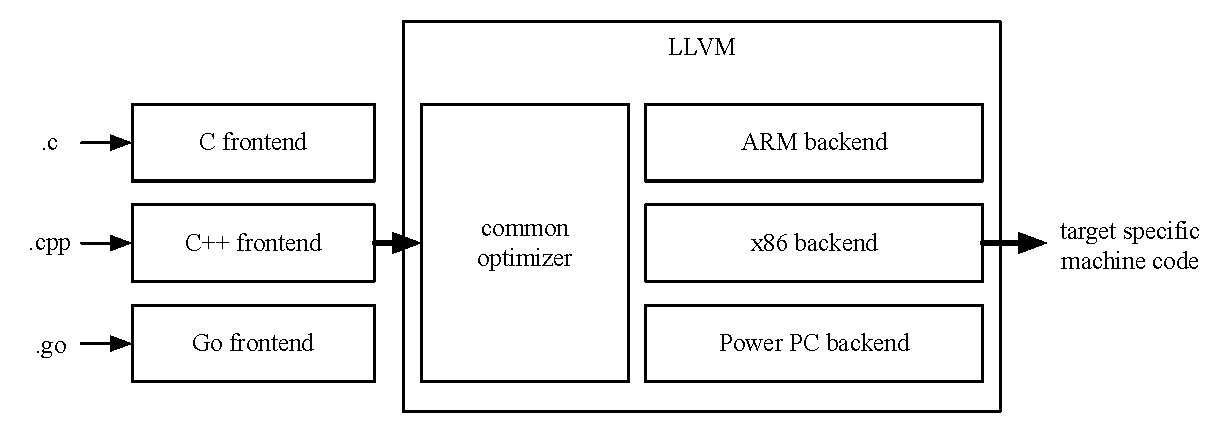
\includegraphics[width=10cm]{./figs/llvm}
\caption{LLVM}
\label{fig:llvm}
\end{figure}

Desarrollamos la NVM basándonos en LLVM (véase \reffig{fig:nvm}). En primer lugar, proporcionamos las librerías API subyacentes para blockchain. Luego, creamos un \textit{frontend} para el compilador, disponible en diferentes lenguajes tales como Solidity, JavaScript, C, C++, Go, etc. A continuación, utilizamos el \textit{toolchain} proporcionado por LLVM para generar el bytecode LLVM. Finalmente, este bytecode LLVM se ejecuta en un \textit{sandbox} proporcionado por NVM a través del motor JIT de LLVM.

\begin{figure}[h]
\centering
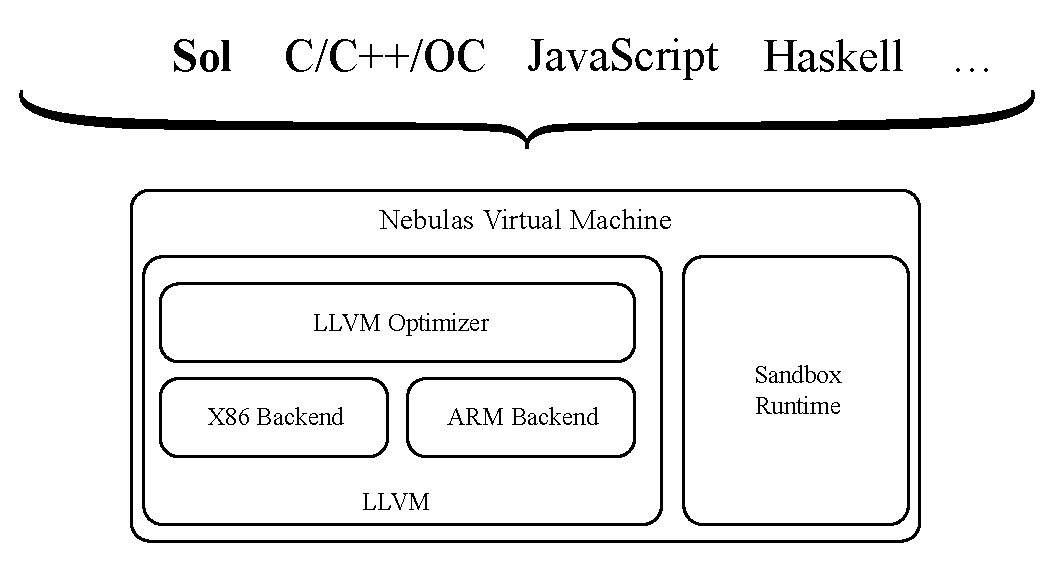
\includegraphics[width=10cm]{./figs/nvm}
\caption{Máquina Virtual de Nebulas}
\label{fig:nvm}
\end{figure}

La Máquina Virtual de Nebulas es la piedra angular de Nebulas Force. Cuando se libera un nuevo código de protocolo o un contrato inteligente, el bytecode LLVM se genera luego de que el nuevo código es compilado por LLVM en NVM, y es liberado al blockchain. Una vez confirmado allí, el nuevo código será compilado y optimizado por LLVM JIT, y colocado en el sandbox para reemplazar el código viejo y ser ejecutado, tal como se muestra en la \reffig{fig:nvm-process}.

\begin{figure}[h]
\centering
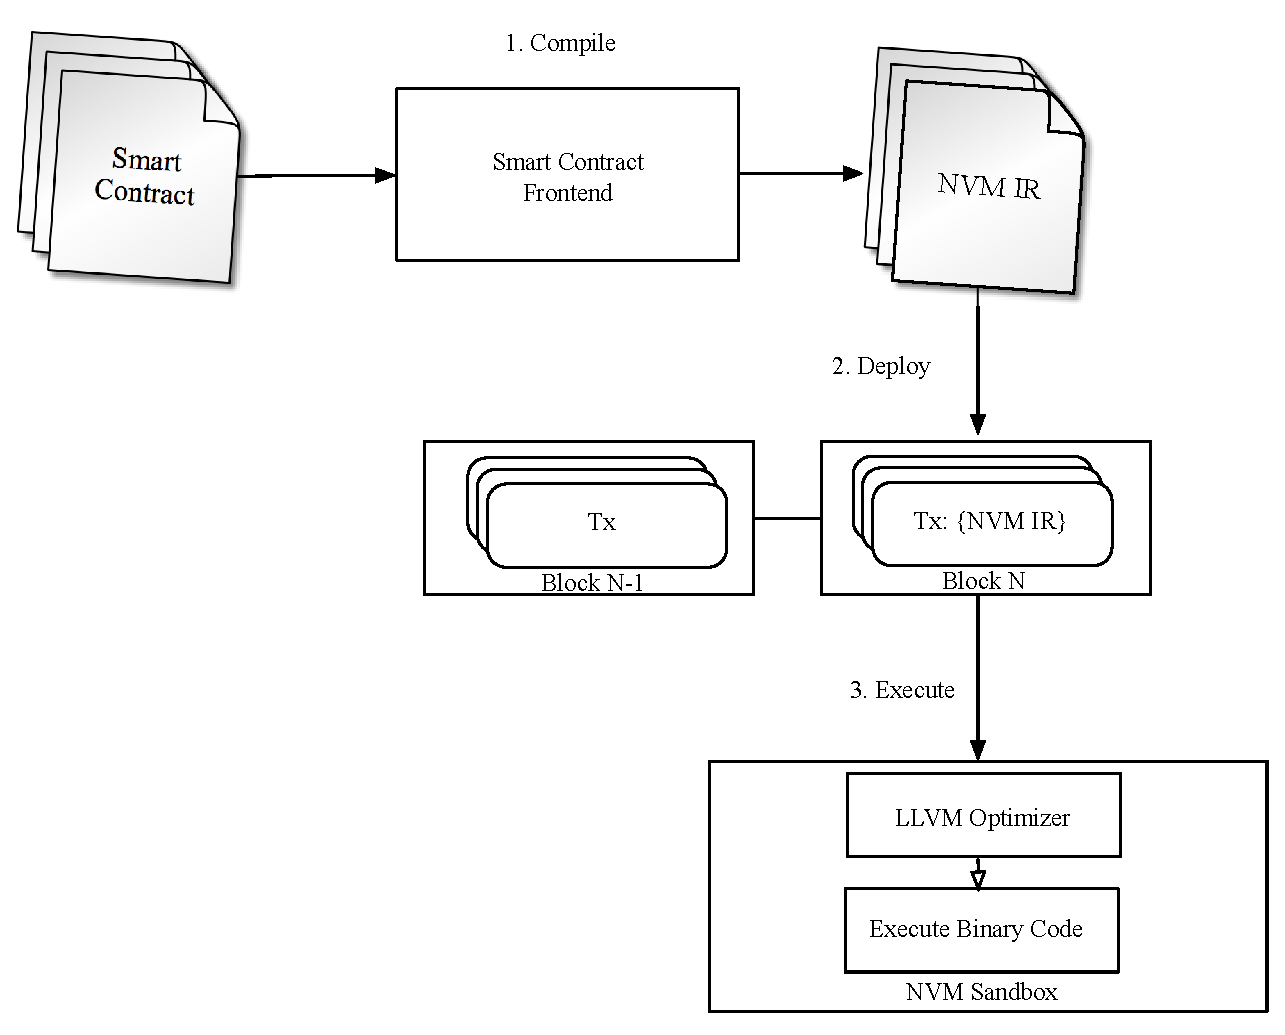
\includegraphics[width=10cm]{./figs/nvm-process}
\caption{El mecanismo de operación de la Máquina Virtual de Nebulas}
\label{fig:nvm-process}
\end{figure}

Con LLVM (véase \reffig{fig:llvm}), NVM también ayuda a los desarrolladores a escribir contratos y aplicaciones inteligentes por medio de sus lenguajes de programación favoritos, como Solidity, JavaScript, e incluso Haskell. Además de estos populares lenguajes, NVM también da soporte a lenguajes personalizados de alto nivel para diferentes áreas y escenarios, tales como DSL para sistemas financieros. Estos lenguajes de alto nivel son más fáciles de verificar formalmente, mejorando aún más la robustez y seguridad del código, algo que permite a los desarrolladores escribir contratos y aplicaciones más sofisticadas.
\section{区块和交易}

\todo{Wenbo}

\subsection{Upgrade Design of the Smart Contract}
%\subsection{智能合约的升级设计}

\subsubsection{Turing Complete Smart Contract Programming Language}
%\subsubsection{图灵完备的智能合约编程语言}

A smart contract is a set of promises defined in the digital form, including agreements for the execution of those promises by the contract participants. Physically, the carrier of the smart contract is the computer code that the computer can recognize and can be operated on the computer. Bitcoin script language is an imperative and stack-based programming language, and because it is Turing incomplete, there are some limitations on its applications. The Ethereum is the world's first blockchain system that implements Turing complete smart contracts. The adopted programming language is Solidity and Serpent, enabling developers to develop a wide variety of applications in a rapid and efficient manner. After the smart contract code is published on the blockchain, it can be automatically executed without participation of any agencies.

%智能合约是一套以数字形式定义的承诺(promises),包括合约参与方可以在上面执行这些承诺的协议。在物理上,智能合约的载体是计算机可识别并运行的计算机代码。比特币脚本语言是一种命令式的、基于栈的编程语言,由于它是非图灵完备的,所以应用上有一定的局限性。以太坊是全世界第一个实现图灵完备的智能合约的区块链系统,编程语言是Solidity、Serpent,使得应用开发者们可以高效快速地开发各式各样的应用程序。智能合约代码发布到区块链上之后,无需中介的参与,在区块链上自动执行。

In the early stage, the smart contract programming language in the Nebulas was fully compatible with Solidity of Ethereum, making it easy for developers to migrate the smart contract applications developed for Ethereum into Nebulas seamlessly. We add some instruction sets related to the Nebulas Rank to Solidity language, facilitating developers to obtain the NR value of any users. After that, based on NVM, we provide support to various programming languages, making it easy for developers to program with their favorite advanced languages, such as Java, Python, Go, JavaScript, Scala, etc., or even create customized applications with certain advanced languages in a specific field. 

%星云链中的智能合约编程语言,在初期时完全兼容以太坊的Solidity,方便开发者为以太坊开发的智能合约应用无缝的迁移到星云链中来。我们在Solidity语言中增加一些跟Nebulas Rank相关的指令集,方便开发者获取任意用户的NR值。后续我们基于NVM推出各种编程语言的支持,使得开发者可以用自己喜欢的高级语言编程,例如Java、Python、Go、JavaScript、Scala等,甚至定制的应用在特定领域的高级语言。

\subsubsection{Upgradable Contracts}
%\subsubsection{合约可升级}

Currently, for the design of the smart contract of Ethereum, once the code is made, it cannot be changed any more. From the moment that the code logic is made, it cannot be upgraded forever. If the smart contract serves as an agreement, it is required to be unchangeable, which represents an agreement that its operation is determined. However, as the smart contract has been increasingly widely used, its workflow and code become more and more complicated. It is found that it looks like a real contract in the real world. If it fails to be reviewed carefully, it is difficult to prevent human errors in the design and coding process. Once hackers find any bugs, the loss is always very significant. In June 2016, the DAO Attack was due to a code defect, causing a total loss of \$60 million to the users of Ethereum. In addition, a recent bug of Parity Wallet resulted in a loss of 150,000 ETH, valued at \$30 million. Since the bitcoin is designed with Turing incompleteness and many script instructions have been deleted, its security level is very high. 

%目前以太坊智能合约的设计是代码一经部署,不可变化,代码逻辑从部署的时刻起,便永远不再具有升级的能力。智能合约如果作为协议来看,不可变化是其要求的,代表着一种协议的约定,运行行为都是确定性的。但是随着智能合约开始获得越来越多的使用,其流程和代码也变得越来越复杂,人们发现,就像现实世界的合同一样,如果没有认真审核的话,在设计和编码过程中难以避免人工失误的产生,一旦被黑客找到漏洞,损失往往是巨大的。2016年6月,The DAO攻击事件,由于一个代码缺陷,导致以太坊用户损失了共计6000万美元的损失;最近Parity钱包的漏洞,导致15万个以太币的流失,价值3000万美元。比特币由于其设计上的非图灵完备性,删减了许多脚本指令,所以其安全性是极高的。

Although there are many premium practices in smart contract programing, more strict reviewing process and even formal verification tools to verify the certainty of the smart contract through mathematical proofs, codes cannot be totally bug-free. When looking back into our currently centralized Internet world, we find that Internet services can be upgraded so as to fix different bugs emerged in the development process. Perfect application system cannot be designed, but is evolved gradually. We believe that the fundamental requirement of sorting out security problem of the smart contract is to formulate an upgradable design solution for the smart contract.

%虽然目前有各种智能合约编程的最佳实践,以及更严格的审核流程,甚至出现形式化验证工具,通过数学证明的方式验证智能合约的确定性。但是既然是代码,就不可能没有漏洞。回顾我们现在的中心化的互联网世界,各种互联网服务都是可以升级的,弥补开发过程中发生的各种漏洞。任何一个完美的应用系统,都是演化而不是设计出来的。我们认为,解决智能合约安全性的根本问题,需要有一个好的智能合约可升级设计方案。

There are some solutions to the upgradeable design of the smart contract in Ethereum, which are generally divided into two categories. The first one is the Proxy Contract available to the public. Its code is very simple, only forwarding the request to the following real function contract. When the contract needs upgrading, just make the pointer of the internal function contract of the Proxy Contract point to the new contract. The second one is to separate the code contract from storage contract. The storage contract is responsible for providing the external contract with methods to read and write the internal state. The code contract is responsible for the real business logic, and when upgrading, it is only responsible for deploying the new code contract so as to lose no state. These two solutions have their own limitations correspondingly, so they cannot solve all the problems. For example, the separation between the code contract and storage contract makes it more complicated. Sometimes it is even unfeasible. Although the Proxy Contract is able to point to the new contract, the state data of the old contract cannot be migrated. Some contracts are not well designed at the initial development stage, so they fail to leave any interface for later upgrade.

%以太坊上的智能合约可升级设计有一些解决方案,大体上分为两类:一类是对外公开代理合约 (Proxy Contract),代理合约的代码非常简单,仅仅把请求转发给后面的真正的功能合约。当需要升级合约时,把代理合约的内部功能合约指针指向新的合约即可;第二类是把合约的代码和存储分离,存储合约负责提供方法,供外部合约读写内部状态,代码合约做真正的业务逻辑,升级时只需要部署新的代码合约,不丢失所有的状态。这两类方案都有其局限性,不能解决所有问题:合约的代码和存储分离在设计上增加了很多复杂度,有时候甚至不可行;代理合约虽然能够指向新合约,但是老合约的状态数据并不能迁移;有些合约在开始开发时,没有良好的设计,没有为以后的升级留下接口。

We designed a simple smart contract upgrade solution. In this way, at the language level, another contract can read and write a contract state variable directly (in line with the security constraints). For example, there is a Token contract, and its code is as shown in Table \ref{figure:nf:oldsc}. \\

%我们设计一种简洁的智能合约升级方案:在语言层面上,我们支持一个合约的状态变量供另外一个合约直接读写(符合安全约束)。这是一个例子,假如有个Token合约,代码如表\ref{figure:nf:oldsc}所示。

	\begin{figure}[!h]
  	\centering
  	\begin{minipage}{0.95\linewidth}
	\begin{lstlisting}[frame=single]
contract Token {
  mapping (address => uint256) balances shared;

  function transfer(address _to, uint256 _value) returns (bool success) {
     if (balances[msg.sender] >= _value) {
       balances[msg.sender] -= _value;
       balances[_to] += _value;
       return true;
     } else {
       return false;
     }
   }
   function balanceOf(address _owner) constant returns (uint256 balance) {
       return balances[_owner];
   }
}
	\end{lstlisting}
  	\end{minipage}
  	\caption{Original Contract Code}
  	\label{figure:nf:oldsc}
	\end{figure}

When the contract is deployed, the balances variable is marked with the keyword of shared, and when it is compiled into bytecode for operation, the virtual machine will design the storage area separately for this variable. For the variable that is not marked with the keyword of shared, it cannot be accessed directly by other contracts.

%合约部署时,balances变量用关键字shared标识,编译成字节码运行时,虚拟机会为该变量单独设计存储区域。不用关键字shared声明的变量,都不可以被其它合约直接访问。

If a bug in the transfer function of the original code needs modifying, check the \_value and deploy the new smart contract code as shown in Table \ref{figure:nf:newsc}.

%假如原代码的transfer函数需要修改一个bug,对\_value做检查,部署新的智能合约代码,如表\ref{figure:nf:newsc}所示。

	\begin{figure}[!h]
  	\centering
  	\begin{minipage}{0.95\linewidth}
	\begin{lstlisting}[frame=single]
[baseContractAddress="0x5d65d971895edc438f465c17db6992698a52318d"]
//baseContractAddress is the address of the old contract
contract Token {
  mapping (address => uint256) balances shared;

  function transfer(address _to, uint256 _value) returns (bool success) {
     if (balances[msg.sender] >= _value ^&& _value > 0^) {
       balances[msg.sender] -= _value;
       balances[_to] += _value;
       return true;
     } else {
       return false;
     }
   }
   function balanceOf(address _owner) constant returns (uint256 balance) {
       return balances[_owner];
   }
}
	\end{lstlisting}
  	\end{minipage}
  	\caption{New Contract Code}
  	\label{figure:nf:newsc}
	\end{figure}

After the new contract is deployed, the old contract can choose selfdestruct, which means that it cannot be accessed any more. But the shared variable will be permanently reserved. The new contract can completely inherit the asset of balances from the old contract without losing any state, so no additional migration is required. However, when developing a smart contract, it is necessary to declare the critical state variable to be shared. The compiler will specially handle the storage area of the variable so as to ensure that it can be accessed by other authorized contracts.

%新的合约部署以后,老的合约可以选择selfdestruct,不能再被访问,但是shared变量依然被永久保留。新的合约可以完全继承老合约的balances资产,全部的状态都不丢失,不需要做额外的迁移工作。但是在开发智能合约时,对关键的状态变量声明为shared是必须的,编译器会对变量的存储区域做特殊处理,保证其可以被其它授权的合约访问。

In order to ensure the security, the contract upgrade and the old contract must use the same creator, otherwise an exception will be thrown during operation. 

%为了保证安全,升级合约和老合约必须是相同的creator,否则运行时会抛异常。

There is a moral problem in this design. Once the provisions of the contract has been proposed and concluded, they should not be modified. Any change later should be agreed by the contract audiences. We plan to introduce a voting mechanism to approve the upgrade of the smart contract, preventing the contract from being modified silently by the contract creator. 

%这种设计存在道德上的问题,因为合约的内容条款一旦拟订,其实是不应该被修改的,至少修改必须征询合约受众的同意。我们计划引入投票机制,以批准智能合约的升级,而不是默默的被合约创建者修改。

With this upgradable solution, the DAO Attack or Parity bug or similar bug attack events can be fixed more rapidly, rather than through hard fork. After repair, assets of all users can continue to be used without migration.

%通过这种可升级方案,The DAO或者Parity类似的漏洞攻击事件,可以更快的被修复,而不是通过硬分叉的方式。并且修复以后,所有用户的资产都不需要迁移,仍然继续使用。



